% =============================================================================
% cuda_learning_material.tex
% Learning Material: CUDA GPU Parallelism
% EC7207 High Performance Computing – Group 11
% =============================================================================
\documentclass[12pt,a4paper]{article}

\usepackage[margin=2.5cm]{geometry}
\usepackage{listings}
\usepackage{xcolor}
\usepackage{amsmath}
\usepackage{booktabs}
\usepackage{hyperref}
\usepackage{tikz}
\usepackage{array}
\usepackage{enumitem}
\usepackage{fancyhdr}
\usepackage{titlesec}

\lstdefinestyle{cudastyle}{
    language=C++,
    basicstyle=\ttfamily\small,
    keywordstyle=\color{blue}\bfseries,
    commentstyle=\color{gray}\itshape,
    stringstyle=\color{red!70!black},
    numbers=left, numberstyle=\tiny\color{gray},
    numbersep=8pt, frame=single, rulecolor=\color{black!30},
    breaklines=true, showstringspaces=false,
    backgroundcolor=\color{gray!5},
    tabsize=4,
    morekeywords={__global__,__device__,__shared__,__host__,
                  blockIdx,blockDim,threadIdx,gridDim,
                  cudaMalloc,cudaFree,cudaMemcpy,
                  cudaMemcpyHostToDevice,cudaMemcpyDeviceToHost,
                  cudaDeviceSynchronize,cudaEventCreate,
                  cudaEventRecord,cudaEventSynchronize,
                  cudaEventElapsedTime,dim3}
}
\lstset{style=cudastyle}

\pagestyle{fancy}
\fancyhf{}
\lhead{EC7207 HPC – Group 11}
\rhead{CUDA — GPU Parallelism}
\cfoot{\thepage}

\titleformat{\section}{\large\bfseries}{}{0em}{}[\titlerule]
\titleformat{\subsection}{\normalsize\bfseries}{}{0em}{}

% =============================================================================
\begin{document}
% =============================================================================

\begin{center}
    {\LARGE\bfseries CUDA — GPU Massively Parallel Computing}\\[0.5em]
    {\large Learning Material for EC7207 High Performance Computing}\\[0.3em]
    {\normalsize Group 11 — Pearson Correlation Recommender System}
\end{center}
\vspace{1em}\hrule\vspace{1.5em}

% =============================================================================
\section{What is CUDA?}
% =============================================================================

\textbf{CUDA} (Compute Unified Device Architecture) is NVIDIA's parallel
computing platform that lets you write C/C++ functions called \textbf{kernels}
that execute on thousands of GPU threads simultaneously.

\subsection{CPU vs.\ GPU: Two Different Philosophies}

\begin{center}
\begin{tabular}{lll}
\toprule
Feature & CPU & GPU \\
\midrule
Core count & 4--64 powerful cores & 1,000s of simple cores \\
Clock speed & 3--5 GHz & 1--2 GHz \\
Cache per core & Large L1/L2/L3 & Small \\
Branch prediction & Sophisticated & Minimal \\
Best for & Complex sequential logic & Data-parallel repetitive work \\
Memory bandwidth & $\sim$50--100 GB/s & $\sim$400--2000 GB/s \\
\bottomrule
\end{tabular}
\end{center}

\textbf{Why is our problem a perfect GPU fit?}  Computing the Pearson
similarity between any two users $(u,v)$ is completely independent of any
other pair.  We have $N^2 = 1{,}000{,}000$ independent computations —
exactly the kind of \emph{embarrassingly parallel} workload GPUs excel at.

% =============================================================================
\section{CUDA Thread Hierarchy}
% =============================================================================

CUDA organises threads in a three-level hierarchy.  You must understand this
to write any CUDA kernel:

\subsection{Thread}
The smallest execution unit.  Each thread:
\begin{itemize}
    \item Runs the kernel function independently
    \item Has its own \textbf{registers} (fastest storage)
    \item Has a unique identity: \texttt{threadIdx.x}, \texttt{threadIdx.y},
          \texttt{threadIdx.z}
\end{itemize}

\subsection{Block}
A group of threads (up to 1024) that:
\begin{itemize}
    \item Run on the same \textbf{Streaming Multiprocessor (SM)}
    \item Can share fast \textbf{shared memory} (48 KB per SM)
    \item Can synchronise with \texttt{\_\_syncthreads()}
    \item Have a unique block identity: \texttt{blockIdx.x}, \texttt{blockIdx.y}
    \item Threads in \emph{different} blocks cannot share memory or synchronise
\end{itemize}

\subsection{Grid}
The collection of \emph{all} blocks for one kernel launch.
The GPU scheduler distributes blocks across all SMs automatically.

\subsection{Computing Global Thread Indices}

\begin{lstlisting}
/* 1D kernel (1D grid, 1D block): */
int tid = blockIdx.x * blockDim.x + threadIdx.x;

/* 2D kernel (2D grid, 2D block): */
int row = blockIdx.y * blockDim.y + threadIdx.y;
int col = blockIdx.x * blockDim.x + threadIdx.x;
\end{lstlisting}

\begin{center}
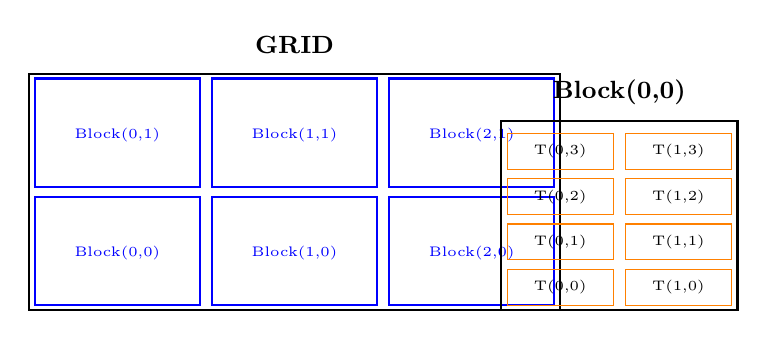
\begin{tikzpicture}[x=1.5cm,y=1.2cm]
    % Grid
    \draw[thick] (0,0) rectangle (4.5,2.5);
    \node[font=\small\bfseries] at (2.25,2.8) {GRID};
    % Blocks
    \foreach \bx in {0,1,2} \foreach \by in {0,1} {
        \draw[blue,thick] (\bx*1.5+0.05,\by*1.25+0.05)
              rectangle (\bx*1.5+1.45,\by*1.25+1.2);
        \node[font=\tiny,blue] at (\bx*1.5+0.75,\by*1.25+0.6)
              {Block(\bx,\by)};
    }
    % Threads inside one block
    \begin{scope}[xshift=6cm]
    \draw[thick] (0,0) rectangle (2,2);
    \node[font=\small\bfseries] at (1,2.3) {Block(0,0)};
    \foreach \tx in {0,1} \foreach \ty in {0,1,2,3} {
        \draw[orange] (\tx+0.05,\ty*0.48+0.05)
              rectangle (\tx+0.95,\ty*0.48+0.43);
        \node[font=\tiny] at (\tx+0.5,\ty*0.48+0.24)
              {T(\tx,\ty)};
    }
    \end{scope}
\end{tikzpicture}
\end{center}

% =============================================================================
\section{GPU Memory Hierarchy}
% =============================================================================

From fastest to slowest access:

\begin{center}
\begin{tabular}{lllp{4.5cm}}
\toprule
Memory & Scope & Size & Access time \\
\midrule
Registers & Per thread & $\sim$255 per thread & $<$1 cycle \\
Shared memory & Per block & $\sim$48 KB per SM & $\sim$1--5 cycles \\
L1 cache & Per SM & $\sim$32--128 KB & $\sim$28 cycles \\
L2 cache & GPU-wide & $\sim$1--40 MB & $\sim$100 cycles \\
Global memory & GPU-wide & GBs (DRAM) & $\sim$300--600 cycles \\
Host memory & CPU RAM & GBs & Via PCIe ($\sim$12 GB/s) \\
\bottomrule
\end{tabular}
\end{center}

\textbf{In our project:}
\begin{itemize}
    \item \texttt{d\_ratings}, \texttt{d\_user\_mean}, \texttt{d\_sim},
          \texttt{d\_pred} live in \textbf{global memory} (GPU DRAM)
    \item Scalar variables inside kernels (\texttt{num}, \texttt{den\_u},
          \texttt{co}, etc.) live in \textbf{registers}
    \item The top-K arrays in the prediction kernel
          (\texttt{top\_sim}, \texttt{top\_rat}, \texttt{top\_mu}, size 20
          each) live in \textbf{registers} — if they don't fit, they spill to
          local memory (slow!)
    \item We don't use shared memory because our kernels are
          \emph{embarrassingly parallel} (no inter-thread cooperation)
\end{itemize}

% =============================================================================
\section{The Three GPU Kernels}
% =============================================================================

\subsection{Kernel 1: \texttt{kernel\_user\_means} — 1D Grid}

\begin{lstlisting}
/* Each thread handles one user row */
__global__ void kernel_user_means(
        const float *ratings, float *user_mean,
        int N_USERS, int N_ITEMS)
{
    int u = blockIdx.x * blockDim.x + threadIdx.x;
    if (u >= N_USERS) return;   /* bounds check */

    double sum = 0.0; int cnt = 0;
    for (int i = 0; i < N_ITEMS; i++) {
        float r = ratings[u * N_ITEMS + i];
        if (r != 0.0f) { sum += r; cnt++; }
    }
    user_mean[u] = (cnt > 0) ? (float)(sum / cnt) : 3.0f;
}

/* Launch: one thread per user */
int blocks = (N_USERS + 255) / 256;
kernel_user_means<<<blocks, 256>>>(d_ratings, d_user_mean, N_USERS, N_ITEMS);
\end{lstlisting}

\textbf{Grid layout:} \texttt{blocks}$\times$256 threads total.  Thread $k$
handles user $k$.  The \texttt{if (u >= N\_USERS) return;} guard handles
cases where $N_{\text{USERS}}$ is not a multiple of 256.

\subsection{Kernel 2: \texttt{kernel\_similarity} — 2D Grid}

\begin{lstlisting}
__global__ void kernel_similarity(
        const float *ratings, const float *user_mean,
        float *sim, int N_USERS, int N_ITEMS)
{
    int u = blockIdx.x * blockDim.x + threadIdx.x;
    int v = blockIdx.y * blockDim.y + threadIdx.y;
    if (u >= N_USERS || v >= N_USERS) return;

    if (u == v) { sim[u * N_USERS + v] = 1.0f; return; }
    if (u > v)  return;  /* upper triangle only */

    /* ... compute Pearson correlation ... */
    float s = (float)(num / denom);
    if (s >  1.0f) s =  1.0f;
    if (s < -1.0f) s = -1.0f;
    sim[u * N_USERS + v] = s;
    sim[v * N_USERS + u] = s;  /* mirror -- race-free: unique (u,v) pair */
}

/* Launch: 2D grid of 16x16 thread blocks */
dim3 block(16, 16);  /* 256 threads per block */
dim3 grid((N_USERS + 15) / 16, (N_USERS + 15) / 16);
kernel_similarity<<<grid, block>>>(d_ratings, d_user_mean, d_sim, N_USERS, N_ITEMS);
\end{lstlisting}

\textbf{Why 2D grid?}  The similarity matrix is 2D (u,v).  A 2D grid maps
thread $(tx, ty)$ directly to matrix position $(u, v)$ — natural and efficient.

\textbf{Upper triangle only:}  With 1000 users, the full grid launches
$\lceil1000/16\rceil^2 = 63^2 = 3969$ blocks.  About half the threads
(lower triangle) return immediately after the \texttt{if (u > v) return;}
check.  The wasted warps are \emph{masked off} by the hardware — some
throughput loss but simpler code.

\subsection{Kernel 3: \texttt{kernel\_predictions} — 2D Grid, Register Top-K}

\begin{lstlisting}
__global__ void kernel_predictions(
        const float *ratings, const float *user_mean,
        const float *sim, float *pred,
        int N_USERS, int N_ITEMS, int TOP_K)
{
    int u    = blockIdx.y * blockDim.y + threadIdx.y;
    int item = blockIdx.x * blockDim.x + threadIdx.x;
    if (u >= N_USERS || item >= N_ITEMS) return;

    /* In-register min-heap for top-K: avoids qsort (unavailable in kernels) */
    float top_sim[20], top_rat[20], top_mu[20];
    float worst = -1.0f; int worst_j = 0; int cnt = 0;

    for (int v = 0; v < N_USERS; v++) {
        if (v == u) continue;
        float rv = ratings[v * N_ITEMS + item];
        if (rv == 0.0f) continue;
        float s = sim[u * N_USERS + v];
        if (s <= 0.0f) continue;

        if (cnt < TOP_K) {
            top_sim[cnt] = s; top_rat[cnt] = rv;
            top_mu[cnt]  = user_mean[v]; cnt++;
            if (cnt == TOP_K) { /* find initial worst */
                worst = top_sim[0]; worst_j = 0;
                for (int j = 1; j < TOP_K; j++)
                    if (top_sim[j] < worst) { worst = top_sim[j]; worst_j = j; }
            }
        } else if (s > worst) {
            top_sim[worst_j] = s; top_rat[worst_j] = rv;
            top_mu[worst_j]  = user_mean[v];
            worst = top_sim[0]; worst_j = 0;
            for (int j = 1; j < TOP_K; j++)
                if (top_sim[j] < worst) { worst = top_sim[j]; worst_j = j; }
        }
    }
    /* ... weighted average using top_sim/top_rat/top_mu ... */
}
\end{lstlisting}

\textbf{Why not \texttt{qsort}?}  \texttt{qsort} is a CPU library function
not available in GPU device code (\texttt{\_\_global\_\_} and
\texttt{\_\_device\_\_} functions).  We implement an \emph{in-register
min-heap}: maintain the current worst element of the top-K list and replace
it whenever a better neighbour is found.

\textbf{Register pressure:}  \texttt{top\_sim[20]}, \texttt{top\_rat[20]},
\texttt{top\_mu[20]} = 60 floats $\times$ 4 bytes = 240 bytes per thread.  A
GPU SM has $\sim$65,536 32-bit registers (256 KB), shared across all resident
threads.  If each thread uses 60 registers, a 256-thread block uses 15,360
registers — well within limits.  The compiler may spill to local memory
(slow!) if pressure is too high.

% =============================================================================
\section{Host-Device Memory Management}
% =============================================================================

\begin{lstlisting}
float *d_ratings, *d_user_mean, *d_sim, *d_pred;

/* Allocate on GPU */
cudaMalloc(&d_ratings,  N_USERS * N_ITEMS * sizeof(float));
cudaMalloc(&d_user_mean, N_USERS * sizeof(float));
cudaMalloc(&d_sim,      N_USERS * N_USERS * sizeof(float));
cudaMalloc(&d_pred,     N_USERS * N_ITEMS * sizeof(float));

/* Copy data from CPU to GPU */
cudaMemcpy(d_ratings, h_ratings,
           N_USERS * N_ITEMS * sizeof(float),
           cudaMemcpyHostToDevice);

/* Launch kernels... */

/* Copy results from GPU back to CPU */
cudaMemcpy(h_sim_matrix, d_sim,
           N_USERS * N_USERS * sizeof(float),
           cudaMemcpyDeviceToHost);

/* Free GPU memory */
cudaFree(d_ratings); cudaFree(d_user_mean);
cudaFree(d_sim);     cudaFree(d_pred);
\end{lstlisting}

\textbf{CUDA\_CHECK macro} — every CUDA API call should be wrapped:
\begin{lstlisting}
#define CUDA_CHECK(call) do { \
    cudaError_t e = (call); \
    if (e != cudaSuccess) { \
        fprintf(stderr, "CUDA error %s:%d: %s\n", \
                __FILE__, __LINE__, cudaGetErrorString(e)); \
        exit(EXIT_FAILURE); \
    } } while(0)

CUDA_CHECK(cudaMalloc(&d_ratings, N_USERS * N_ITEMS * sizeof(float)));
\end{lstlisting}

% =============================================================================
\section{Timing GPU Kernels: CUDA Events}
% =============================================================================

\begin{lstlisting}
cudaEvent_t ev_start, ev_stop;
cudaEventCreate(&ev_start);
cudaEventCreate(&ev_stop);

cudaEventRecord(ev_start);           /* mark start */
kernel_similarity<<<grid, block>>>(...);
cudaEventRecord(ev_stop);            /* mark stop  */

cudaEventSynchronize(ev_stop);       /* wait for GPU to finish */
float ms = 0.0f;
cudaEventElapsedTime(&ms, ev_start, ev_stop);
printf("[Timing] Similarity matrix : %.4f s\n", ms / 1000.0f);
\end{lstlisting}

\textbf{Why not \texttt{clock\_gettime()}?}
\begin{itemize}
    \item CUDA kernel launches are \textbf{asynchronous} — \texttt{kernel<<<>>>}
          returns immediately while the GPU runs in the background.
    \item \texttt{clock\_gettime()} on the CPU would measure only the tiny
          launch overhead, not the actual GPU computation time.
    \item CUDA events are timestamps inserted into the GPU command stream,
          measured by the GPU's own clock — they capture true GPU execution time.
\end{itemize}

% =============================================================================
\section{Warps and SIMT Execution}
% =============================================================================

A GPU block's threads are grouped into \textbf{warps} of 32 threads.
All 32 threads in a warp execute the \emph{same instruction} at the
\emph{same time} — this is called \textbf{SIMT (Single Instruction,
Multiple Threads)}.

\subsection{Warp Divergence}

If threads in the same warp take different branches of an \texttt{if}
statement, the warp must execute \emph{both} branches serially with some
threads masked off:

\begin{center}
\begin{tabular}{ll}
\toprule
Scenario & Throughput \\
\midrule
All 32 threads take the same branch & 100\% \\
16 take branch A, 16 take branch B & 50\% (execute A then B) \\
8 threads: each a different branch & 12.5\% \\
\bottomrule
\end{tabular}
\end{center}

In \texttt{kernel\_similarity}, the check \texttt{if (u > v) return;} causes
divergence for threads on the diagonal.  This is acceptable because the
diagonal occupies only $\sim$1\% of the grid (diagonal blocks vs.\ all blocks).

% =============================================================================
\section{Memory Coalescing}
% =============================================================================

GPU global memory accesses are efficient when \textbf{adjacent threads access
adjacent memory addresses} (coalesced access).  The GPU serves the entire
warp with one memory transaction.

\textbf{Our access pattern in \texttt{kernel\_similarity}:}
\begin{itemize}
    \item Thread $(u, v)$ reads \texttt{ratings[u * N\_ITEMS + i]} for all $i$.
          Threads with the same $u$ (same row, consecutive $v$) read different
          \emph{rows} — not coalesced within a row scan.
    \item However, threads in the same warp that process different $(u,v)$
          pairs \emph{do} access different rows, which are spread in memory.
          Full coalescing is hard to achieve for this algorithm.
    \item This is an inherent limitation of the Pearson workload: each thread
          reads one full row of the ratings matrix independently.
\end{itemize}

% =============================================================================
\section{Kernel Launch Syntax}
% =============================================================================

\begin{center}
\texttt{kernelName\textless\textless\textless gridDim, blockDim, sharedMem, stream\textgreater\textgreater\textgreater(args);}
\end{center}

\begin{center}
\begin{tabular}{ll}
\toprule
Parameter & What it specifies \\
\midrule
\texttt{gridDim} & Number of blocks (can be \texttt{int} or \texttt{dim3}) \\
\texttt{blockDim} & Threads per block (can be \texttt{int} or \texttt{dim3}) \\
\texttt{sharedMem} & Extra shared memory per block in bytes (default 0) \\
\texttt{stream} & CUDA stream for asynchronous execution (default 0) \\
\bottomrule
\end{tabular}
\end{center}

\textbf{dim3} allows 3D dimensions:
\begin{lstlisting}
dim3 block(16, 16, 1);   /* 16x16x1 = 256 threads per block */
dim3 grid(64, 64, 1);    /* 64x64 = 4096 blocks */
kernel<<<grid, block>>>(...);
\end{lstlisting}

% =============================================================================
\section{How to Get and Run CUDA}
% =============================================================================

\begin{verbatim}
# Check if NVIDIA GPU is present
nvidia-smi

# Check CUDA compiler version
nvcc --version

# Compile
nvcc -O2 -arch=sm_75 -o cuda_rec cuda/cuda_recommender.cu -lm
# sm_75 = Turing architecture (RTX 20xx, Tesla T4)
# sm_86 = Ampere (RTX 30xx, A100)
# sm_89 = Ada Lovelace (RTX 40xx)

# Run
./cuda_rec 1000 1000
\end{verbatim}

\begin{center}
\begin{tabular}{ll}
\toprule
GPU Family & Architecture (\texttt{-arch}) \\
\midrule
GTX 10xx (Pascal) & \texttt{sm\_61} \\
RTX 20xx (Turing) & \texttt{sm\_75} \\
RTX 30xx (Ampere) & \texttt{sm\_86} \\
RTX 40xx (Ada) & \texttt{sm\_89} \\
A100 (HPC) & \texttt{sm\_80} \\
\bottomrule
\end{tabular}
\end{center}

% =============================================================================
\section{Key Points to Explain in a Presentation}
% =============================================================================

\begin{enumerate}
    \item \textbf{What is a kernel?}  A C function with \texttt{\_\_global\_\_}
          qualifier that runs on the GPU.  When launched, it executes on
          thousands of GPU threads simultaneously, each independently.
    \item \textbf{How does thread indexing work?}  Thread identity is encoded
          in \texttt{blockIdx} and \texttt{threadIdx}.  Thread maps to data
          via: \texttt{u = blockIdx.x * blockDim.x + threadIdx.x}.
    \item \textbf{Why do we need \texttt{cudaMemcpy}?}  CPU and GPU have
          separate physical memory (CPU RAM and GPU VRAM).  Pointers to CPU
          memory are invalid on the GPU and vice versa.  Data must be
          explicitly transferred.
    \item \textbf{Why is GPU transfer overhead a concern?}  PCIe bandwidth
          ($\sim$12 GB/s) is 30--100$\times$ slower than GPU memory bandwidth.
          For small problems, the transfer cost can exceed the speedup gain.
          Our 1000$\times$1000 matrix transfers $\sim$4 MB — fast enough.
    \item \textbf{Why can't we use qsort in a kernel?}  Device code cannot call
          CPU library functions.  We implement an in-register min-heap instead.
    \item \textbf{What is the expected speedup?}  A modern GPU has
          5000--10000 CUDA cores vs.\ 4--8 CPU cores.  For our embarrassingly
          parallel similarity computation, speedups of $10\times$--$50\times$
          over serial are typical (limited by memory bandwidth and PCIe transfer).
\end{enumerate}

\vfill
\begin{center}
    \small\textit{Group 11 — EC7207 High Performance Computing}
\end{center}

\end{document}
